\documentclass[12pt]{article}

%% Basic document formatting
\usepackage{amsmath, amsthm, amssymb, amsfonts}
\usepackage{mathtools}
\usepackage{xspace}
\usepackage{thmtools}
\usepackage{graphicx}
\usepackage{setspace}
\usepackage{fancyhdr}
\usepackage{titling}
\usepackage[left=0.4in,right=0.4in,top=1in,bottom=1in]{geometry}
\usepackage{float}
\usepackage{hyperref}
\usepackage{mathrsfs}
\usepackage{tabularx}
\usepackage[utf8]{inputenc}
\usepackage[english]{babel}
\usepackage{framed}
\usepackage[dvipsnames]{xcolor}
\usepackage{environ}
\usepackage{tcolorbox}
\tcbuselibrary{theorems,skins,breakable}

\usepackage{enumitem}
\setlist[enumerate]{leftmargin=*}
\setlist[enumerate,1]{labelindent=\parindent}
\setlist[enumerate,2]{labelindent=0pt}

% Blackboard Bold
\newcommand{\Z}{\mathbb{Z}}                 % integers
\newcommand{\Zpl}{\mathbb{Z}_{+}}           % positive integers
\newcommand{\Znn}{\mathbb{Z}_{\geq 0}}      % nonnegative integers. 
\newcommand{\Q}{\mathbb{Q}}                 % rationals
\newcommand{\Qpl}{\mathbb{Q}_{+}}           % positive Rationals
\newcommand{\R}{\mathbb{R}}                 % reals
\newcommand{\Rpl}{\mathbb{R}_{+}}           % positive Reals
\newcommand{\C}{\mathbb{C}}                 % complex numbers
\newcommand{\F}{\mathbb{F}}                 % field

% Words
\newcommand{\st}{\text{ such that }}
\newcommand{\wrt}{\text{ with respect to }}
\newcommand{\with}{\text{ with }}
\newcommand{\ie}{\text{, i.e. }}
\newcommand*{\ditto}{\text{---}\texttt{"}\text{---}}

% Operators
\newcommand{\abs}[1]{\left|#1\right|}                   % absolute value
\newcommand{\norm}[1]{\abs{\abs{#1}}}
\newcommand{\floor}[1]{\left\lfloor #1 \right\rfloor}   % floor
\newcommand{\ceil}[1]{\left\lceil #1 \right\rceil}      % ceiling
\newcommand{\powset}[1]{\mathscr{P}(#1)}

% Category Theory 
\renewcommand{\hom}{\text{Hom}}
\newcommand{\homspace}[3]{\hom_{#1}(#2, #3)}
\newcommand{\coproduct}[9]{
  \begin{tikzcd}[ampersand replacement=\&]
      \& \& #1 \arrow[dll, bend right, "#6"] \arrow[dl, "#5"] \\
   #4 \& #3 \arrow[l, "#9"] \\
      \& \& #2 \arrow[ull, bend left, "#8"] \arrow[ul, "#7"]
  \end{tikzcd}
}

\newcommand{\product}[9]{ 
  \begin{tikzcd}[ampersand replacement=\&]
      \& \& #3 \\
      #1 \arrow[r, "#7"] \arrow[urr, bend left, "#5"] \arrow[drr, bend right, "#6"] \& #2 \arrow[ur, "#8"] \arrow[dr, "#9"] \\ 
      \& \& #4
  \end{tikzcd}
}


% Algebra 
\newcommand{\Syl}[2]{\text{Syl}_{#1}{(#2)}}           % set of Sylow-p subgroups 
\newcommand{\<}{\langle}                % \<x\>, subgroup generated by x 
\renewcommand{\>}{\rangle}
\renewcommand{\index}[2]{[#1 : #2]}
\newcommand{\id}{\text{id}}             % identity element
\newcommand{\lhdneq}{%
  \mathrel{\ooalign{$\lneq$\cr\raise.22ex\hbox{$\lhd$}\cr}}}
\newcommand{\order}[1]{\text{o}(#1)}    % order of an element
\newcommand{\spec}{\operatorname{Spec}}
\newcommand{\rad}{\operatorname{rad}}   % radical of an ideal 
\newcommand{\sym}[1]{\mathfrak{S}_{#1}}
\newcommand{\aut}[1]{\text{Aut}(#1)} 
\newcommand{\gal}[2]{\text{Gal}(#1 / #2)} 
\newcommand{\inn}[1]{\text{Inn}(#1)} 
\let\oldcong\cong
\let\oldequiv\equiv
\renewcommand{\cong}{\oldequiv}
\renewcommand{\equiv}{\oldcong}

\newcommand{\triangleleftneq}{\mathrel{\ooalign{%
  $\trianglelefteq$\cr
  \hidewidth\raise0.06ex\hbox{$\not\mkern4mu$}\hidewidth\cr
}}}

\makeatletter % cycle
\newcommand{\cyc}[1]{(\mathbf{\cyc@process#1\relax})}
\def\cyc@process#1#2\relax{%
	#1%
	\ifx\relax#2\relax
	\else
		\,\cyc@process#2\relax
	\fi
}
\makeatother

\newcommand{\GL}[2]{\text{GL}_{#1}(#2)}                             % general linear group
\newcommand{\SL}[2]{\text{SL}_{#1}(#2)}                             % special linear group
\newcommand{\gl}[2]{\mathfrak{gl}_{#1}(#2)}
\renewcommand{\sl}[2]{\mathfrak{sl}_{#1}(#2)}
\newcommand{\so}[2]{\mathfrak{so}_{#1}(#2)}
\newcommand{\su}[1]{\mathfrak{su}(#1)}

% Linear Algebra
\newcommand{\bmat}[1]{\begin{bmatrix}#1\end{bmatrix}}   % bracketed matrix
\newcommand{\rank}{\operatorname{rank}}                 % rank
\newcommand{\nullity}{\operatorname{nullity}}           % nullity
\newcommand{\tr}{\operatorname{tr}}

% Combinatorics
\newcommand{\qnum}[1]{\left[#1\right]_q}                % q-analog
\newcommand{\qfact}[1]{\left[#1\right]!_q}              % q-analog factorial 
\newcommand{\qbinom}[2]{\binom{#1}{#2}_q}               % Gaussian binomial coefficient

% Topology/Analysis
\newcommand{\ball}[2]{\text{B}_{#1}(#2)}  % B_r(x): open r-balls around x
\newcommand{\diam}{\text{diam}}           % diamter of a set in metric space 
\newcommand{\lowint}[2]{\underline{\int_{#1}^{#2}}}
\newcommand{\upint}[2]{\overline{\int}_{#1}^{#2}}

% Misc Notation
\newcommand{\oneton}[1]{\{1, \ldots, #1\}}
\newcommand{\defeq}{\vcentcolon=}   % :=
\newcommand{\eqdef}{=\vcentcolon}   % =: 
\renewcommand{\bf}[1]{\textbf{#1}}
\newcommand{\im}{\operatorname{im}}
\newcommand{\fnrest}[2]{\left.#1\right|_{#2}}
\newcommand{\isom}{\overset{\sim}{\rightarrow}} 


\renewcommand{\thesection}{\arabic{section}.}
\renewcommand{\thesubsection}{(\alph{subsection})}

\newtheorem{claim}{Claim}
\newtheorem{theorem}{Theorem}
\newtheorem{proposition}{Proposition}
\newtheorem*{lemma}{Lemma}

%% Headers & title setup
\newcommand{\course}{Math140C}
\newcommand{\myname}{Jay Ser}
\setlength{\headheight}{14.5pt}
\pagestyle{fancy}
\fancyhf{}
\renewcommand{\headrulewidth}{0.4pt}
\lhead{\course}
\rhead{\myname}
\cfoot{\thepage}
\setlength{\droptitle}{-4em} 
\title{\course\ - HW \#2}
\author{\myname}
\date{2026.04.19} 

\begin{document}
\maketitle
\thispagestyle{fancy}

%------------------------------------------------------------------------------%

\graphicspath{{./img/}}

\newcommand{\Djf}[2]{[D_{#1}#2]}
\newcommand{\grad}[1]{[\nabla #1]}

\section*{Q7}
Suppose for all $x \in E$, 
$$\abs{\Djf{j}{f}(x)} \leq M \hspace{1.5em} (1 \leq j \leq n).$$
Fix $\epsilon > 0$ and let $\delta_0 = \frac{\epsilon}{nM}$. 
Since $E$ is open, pick $\delta < \delta_0$ be the value such that $\ball{\delta}{x} \subset E$. 
Fix $h \in \R^n$ with $\abs{h} < \delta$. 
For each each $j \geq 1$, let $v_j = h_1 e_1 + \ldots + h_j e_j$ and $v_0 = 0$. 
By telescoping, 
\begin{equation} \label{eq:7_telescope}
  f(x + h) - f(x) = \sum_{j = 1}^{n}(f(x + v_j) - f(x + v_{j - 1})).
\end{equation}
For each $j \in \oneton{n}$, define $g_{j}(t) \defeq f(x + v_{j - 1} + te_j h_j)$. 
Since $\ball{\delta}{x} \subset E$ and the ball is convex, $x + v_{j - 1} + t e_j h_j \in E$ for all $t \in [0, 1]$. 
Since $\Djf{j}{f}$ exists for $t \in [0, 1]$, the mean value theorem says there is $\theta_j \in (0, 1)$ such that 
$$g_{j}(1) - g_{j}(0) = h_j \Djf{j}{f}(x + v_{j - 1} + \theta_j h_j e_j)$$
Notice that $g_{j}(1) - g_{j}(0)$ is by definition the $j$th summand in \eqref{eq:7_telescope}. 
Hence 
\begin{align*}
  \abs{f(x + h) - f(x)} & = \abs{\sum_{j = 1}^{n} h_j \Djf{j}{f}(x + v_{j - 1} + \theta_j h_j e_j)} \\ 
                             & \leq \sum_{j = 1}^{n} \abs{h_j} \abs{\Djf{j}{f}(x + v_{j - 1} + \theta_j h_j e_j)} \\ 
                             & \leq nM\abs{h} < \epsilon,
\end{align*}
which shows that $f$ is continuous at $x$. 

\section*{Q9}
Here's a lemma from point-set topology: 
\begin{lemma}
  Let $E$ be a connected metric space. 
  Then $E$ has no proper, nontrivial subset that is both open and closed. 
\end{lemma}
\begin{proof}[Proof of Lemma]
  Suppose $S \subset E$ is both an open and closed subset of $E$. 
  Then $E \setminus S$ is also both open and closed in $E$. 
  $E = S \cup E \setminus S$ and 
  $$S \cap \overline{E \setminus S} = \overline{S} \cap E \setminus S = S \cap E \setminus S = \emptyset.$$
  The connectedness of $E$ forces $S = \emptyset$ or $S = E$. 
\end{proof}

Onto the problem. 
By coroallary 9.19 of Rudin, for all convex subsets $A \subset E$, $f$ is constant on $A$. 
Fix any $a \in E$ and define 
$$S \defeq \{x \in E \st f(a) = f(x)\}.$$
It needs to be shown that $S = E$, and by the lemma, the result will follow if $S$ is nonempty and $S$ is both open and closed in $E$. 
$a \in S$ by definition, so $S$ is not empty. 
Take any $x \in S$. 
Since $E$ is open in $\R^n$, there is an $\epsilon > 0$ such that $\ball{\epsilon}{x} \subset E$. 
This ball is a convex subset of $E$, so $f$ is constant on the ball. 
But by definition of $x$, $f(x) = f(a)$, which shows $\ball{\epsilon}{x} \subset S$. 
By the exact same logic, for any $x \in E \setminus S$, there is an $\epsilon > 0$ such that $\ball{\epsilon}{x} \subset E \setminus S$. 
Hence $S$ is both closed and open in $E$, as was to be shown; 
one concludes $f$ is constant on $E$. 

\section*{Q11}
Fix $x \in \R^n$. 
By definition, 
\begin{align}
  \grad{fg}(x) & \defeq \sum_{j = 1}^{n} \Djf{j}{fg}(x) e_j, \label{eq:11_prodcompact} \\ 
  f(x)\grad{g}(x) + g(x) \grad{f}(x) & \defeq \sum_{j = 1}^{n} \left( f(x) \Djf{j}{g}(x) + g(x) \Djf{j}{f}(x) \right). \label{eq:11_prodexpand}
\end{align}
Because the $e_j$'s are linearly independent, to show $\eqref{eq:11_prodcompact}  = \eqref{eq:11_prodexpand} $,  it suffices to demonstrate that for any coordinate $j \in \oneton{n}$, 
\begin{equation} \label{eq:11_desiredresult}
  \Djf{j}{fg}(x) = f(x) \Djf{j}{g}(x) + g(x) \Djf{j}{f}(x).
\end{equation}
But this follows immediately by the product rule for one-variable functions: 
to see this clearly, let 
\begin{align*}
  \varphi: \R \rightarrow \R; \: & t \mapsto f(x + te_j) \\ 
  \psi: \R \rightarrow \R; \: & t \mapsto g(x + te_j)
\end{align*}
One can write down the limit definition for both the partial derivatives of $f$ and $g$ and the derivatives of $\varphi$ and $\psi$ to see that 
\begin{align*}
  \varphi'(0) & = \Djf{j}{f}(x) \\ 
  \psi'(0) & = \Djf{j}{g}(x)
\end{align*}
Similarly, $(\varphi \psi)'(0) = \Djf{j}{fg}(x)$. 
But also, by the product rule for the derivates of one-variable functions, 
\begin{align*}
  (\varphi \psi)'(0) & = \varphi(0) \psi'(0) + \varphi'(0) \psi(0)  \\ 
                     & = f(x)\Djf{j}{f}(x) + g(x)\Djf{j}{g}(x),
\end{align*}
which gives the desired equality \eqref{eq:11_desiredresult}.

The second identity follows via a parallel analysis. 
It suffices to show $\Djf{j}{\frac{1}{f}}(x) = -f(x)^{2} \Djf{j}{f}(x)$ whenever $f(x) \neq 0$. 
Let 
$$\varphi(t) = f(x + te_j).$$
Then $\varphi(0) \neq 0$ by assumption on $f(x)$, $\Djf{j}{f}(x) = \varphi'(0)$, and $\Djf{j}{\frac{1}{f}}(x) = (\frac{1}{\varphi})'(0)$. 
The quotient rule for single variable functions gives 
$$\left(\frac{1}{\varphi}\right)'(0) = -\frac{\varphi'(0)}{\varphi(0)^2},$$
i.e., $\Djf{j}{\frac{1}{f}}(x) = -\frac{\Djf{j}{f}(x)}{f(x)^2}$. 

\section*{Q12}
\begin{figure}
  \centering
  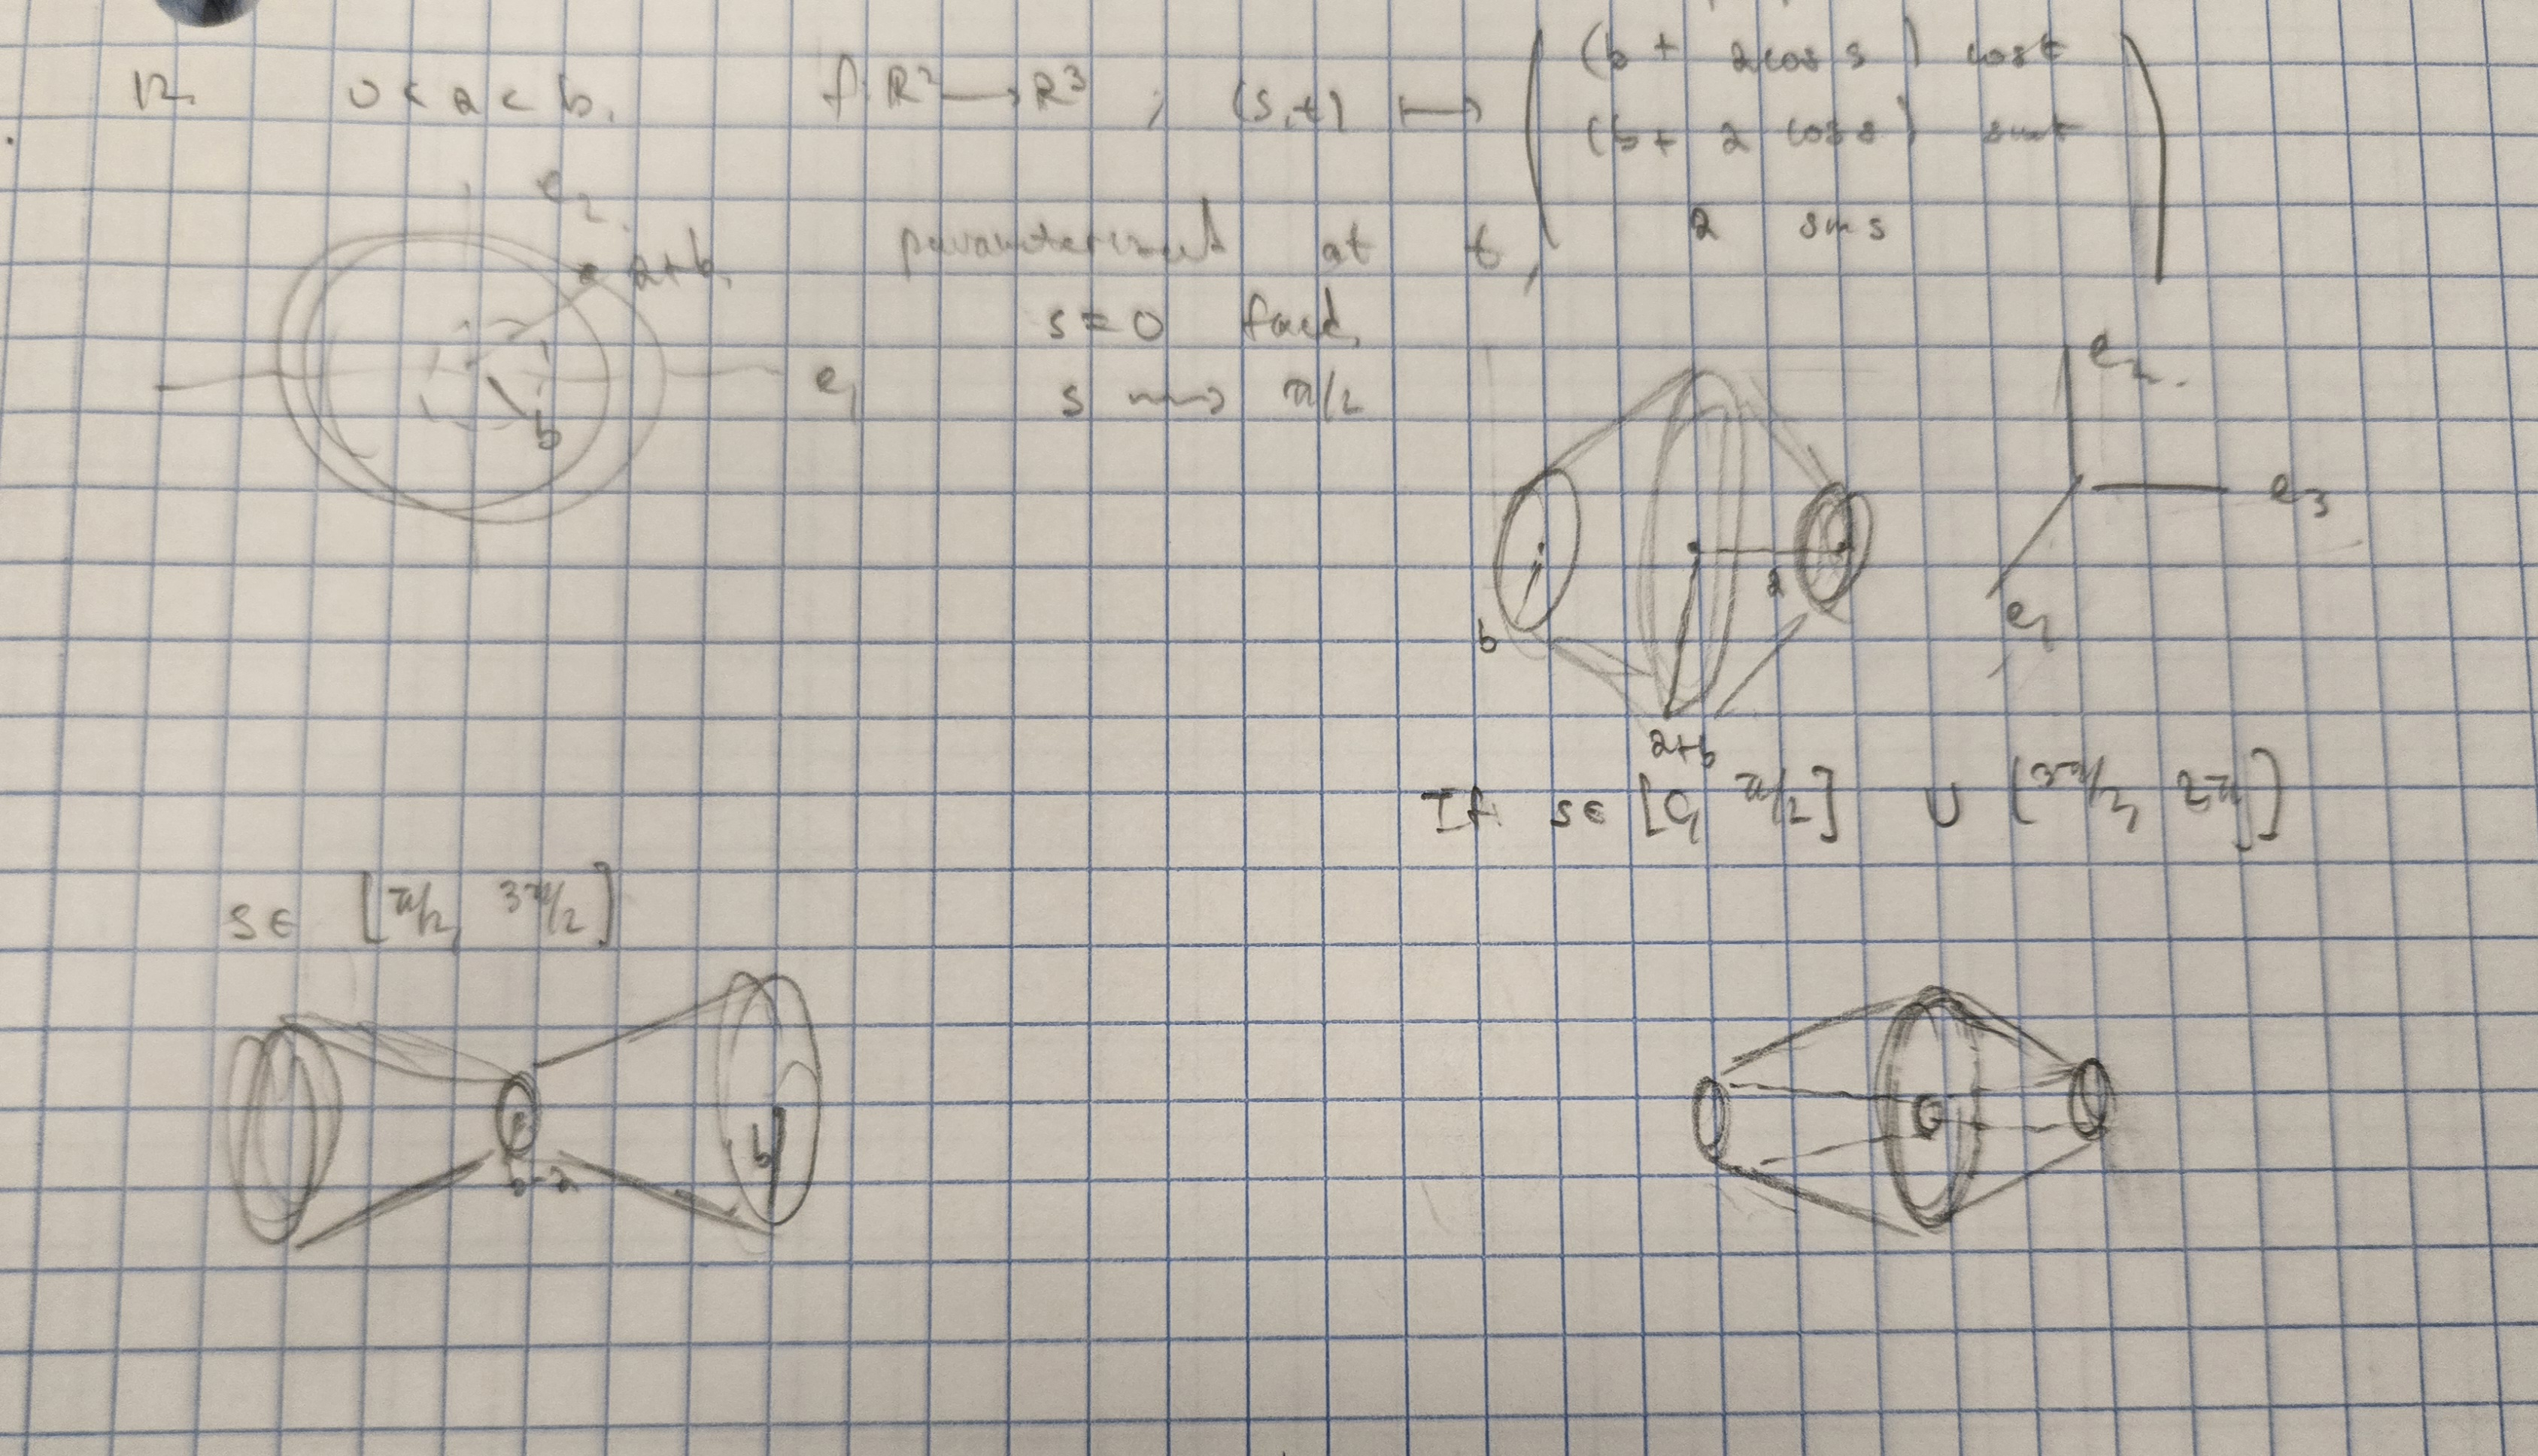
\includegraphics[width=\textwidth]{shapes.jpg}
  \caption{
    Question 12, my attempt to make out the image of $f$.
    When I was drawing this, I made the ``diagonals" of the shape traveling along the $e$ axis to be flat, although in reality, it should be curved a bit like a parabola. 
    Sorry for the blurry image! 
  }
  \label{fig:12_imf}
\end{figure}
I attempt to describe the image of $f$. 
Refer to Figure \ref{fig:12_imf} above.  
Holding $s$ constant at $s = 0$, the image of $f$ is a circle in the $e_1$ and $e_2$ plane of radius $a + b$.
$t$ parameterizes the angle of the point in the circle. 
Hence varying $s$ in $[0, \pi / 2] \cup [3\pi / 2, 2\pi]$ and $t$ in $[0, 2\pi]$ gives a cyclinder-dome thingy, which I will just call a dome.
The ``base" of the dome has radius $a + b$, whereas the ``top" and bottom of the dome has radius $a$. 
Meanwhile, for $s \in [\pi/2, 3\pi/2]$, $f$ produces some kind of inverted dome, as I attempt to demonstrate in the bottom left shape in the figure, where its base has radius $b - a$ and the top has radius $a$.  

\textbf{
  ***Re: I have been told that this shape is actually supposed to be a torus. 
  Darn it!
  I think what I'm describing above is almost like a torus; 
  my illustration on the bottom right is a torus but flipped ``sideways" up.
  It's also a really tall torus, which is what completely threw me off. 
}

\subsection{}
Since $f$ is periodic every $2\pi$, one only needs to consider points on the torus given by $(s, t) \in [0, 2\pi) \times [0, 2\pi)$. 
$$\grad{f_1}(s, t) = \bmat{-a \sin s \cos t \\ -(b + a\cos s)\sin t}$$
So $\grad{f_1}(s, t) = 0$ exactly on the four possible combinations of $s \in \{0, \pi\}$, $t \in \{0, \pi\}$. 
On the torus, these are the points 
\begin{align*}
  (a + b, 0, 0) \\ 
  (- a - b, 0, 0) \\ 
  (b - a, 0, 0) \\ 
  (a - b, 0, 0),
\end{align*}
i.e., the four points of the tori along the $e_1$-axis. 

\subsection{}
$$\grad{f_3}(s, t) = \bmat{a \cos s \\ 0},$$
so $\grad{f_3}(s, t) = 0$ when $s \in \{\pi / 2, 3\pi/2\}$.
On the torus, these are all the points on the ``top" and ``bottom" of the torus (top and bottom when $e_3$ coordinate describes height), 
i.e., the points on the circle given by the cross-section at height $e_3 = a$ and $e_3 = -a$. 

\subsection{}
As described in \textbf{(a)}, the four points in question are the four points that intersect the $e_1$-axis. 
If one draws the torus, one easily sees that the maximum and minimum correspond to the points on the outer radius of the torus, while the saddle points correspond to the inner radius of the torus. 
See Figure \ref{fig:12_torus}.  
\begin{figure}
  \centering
  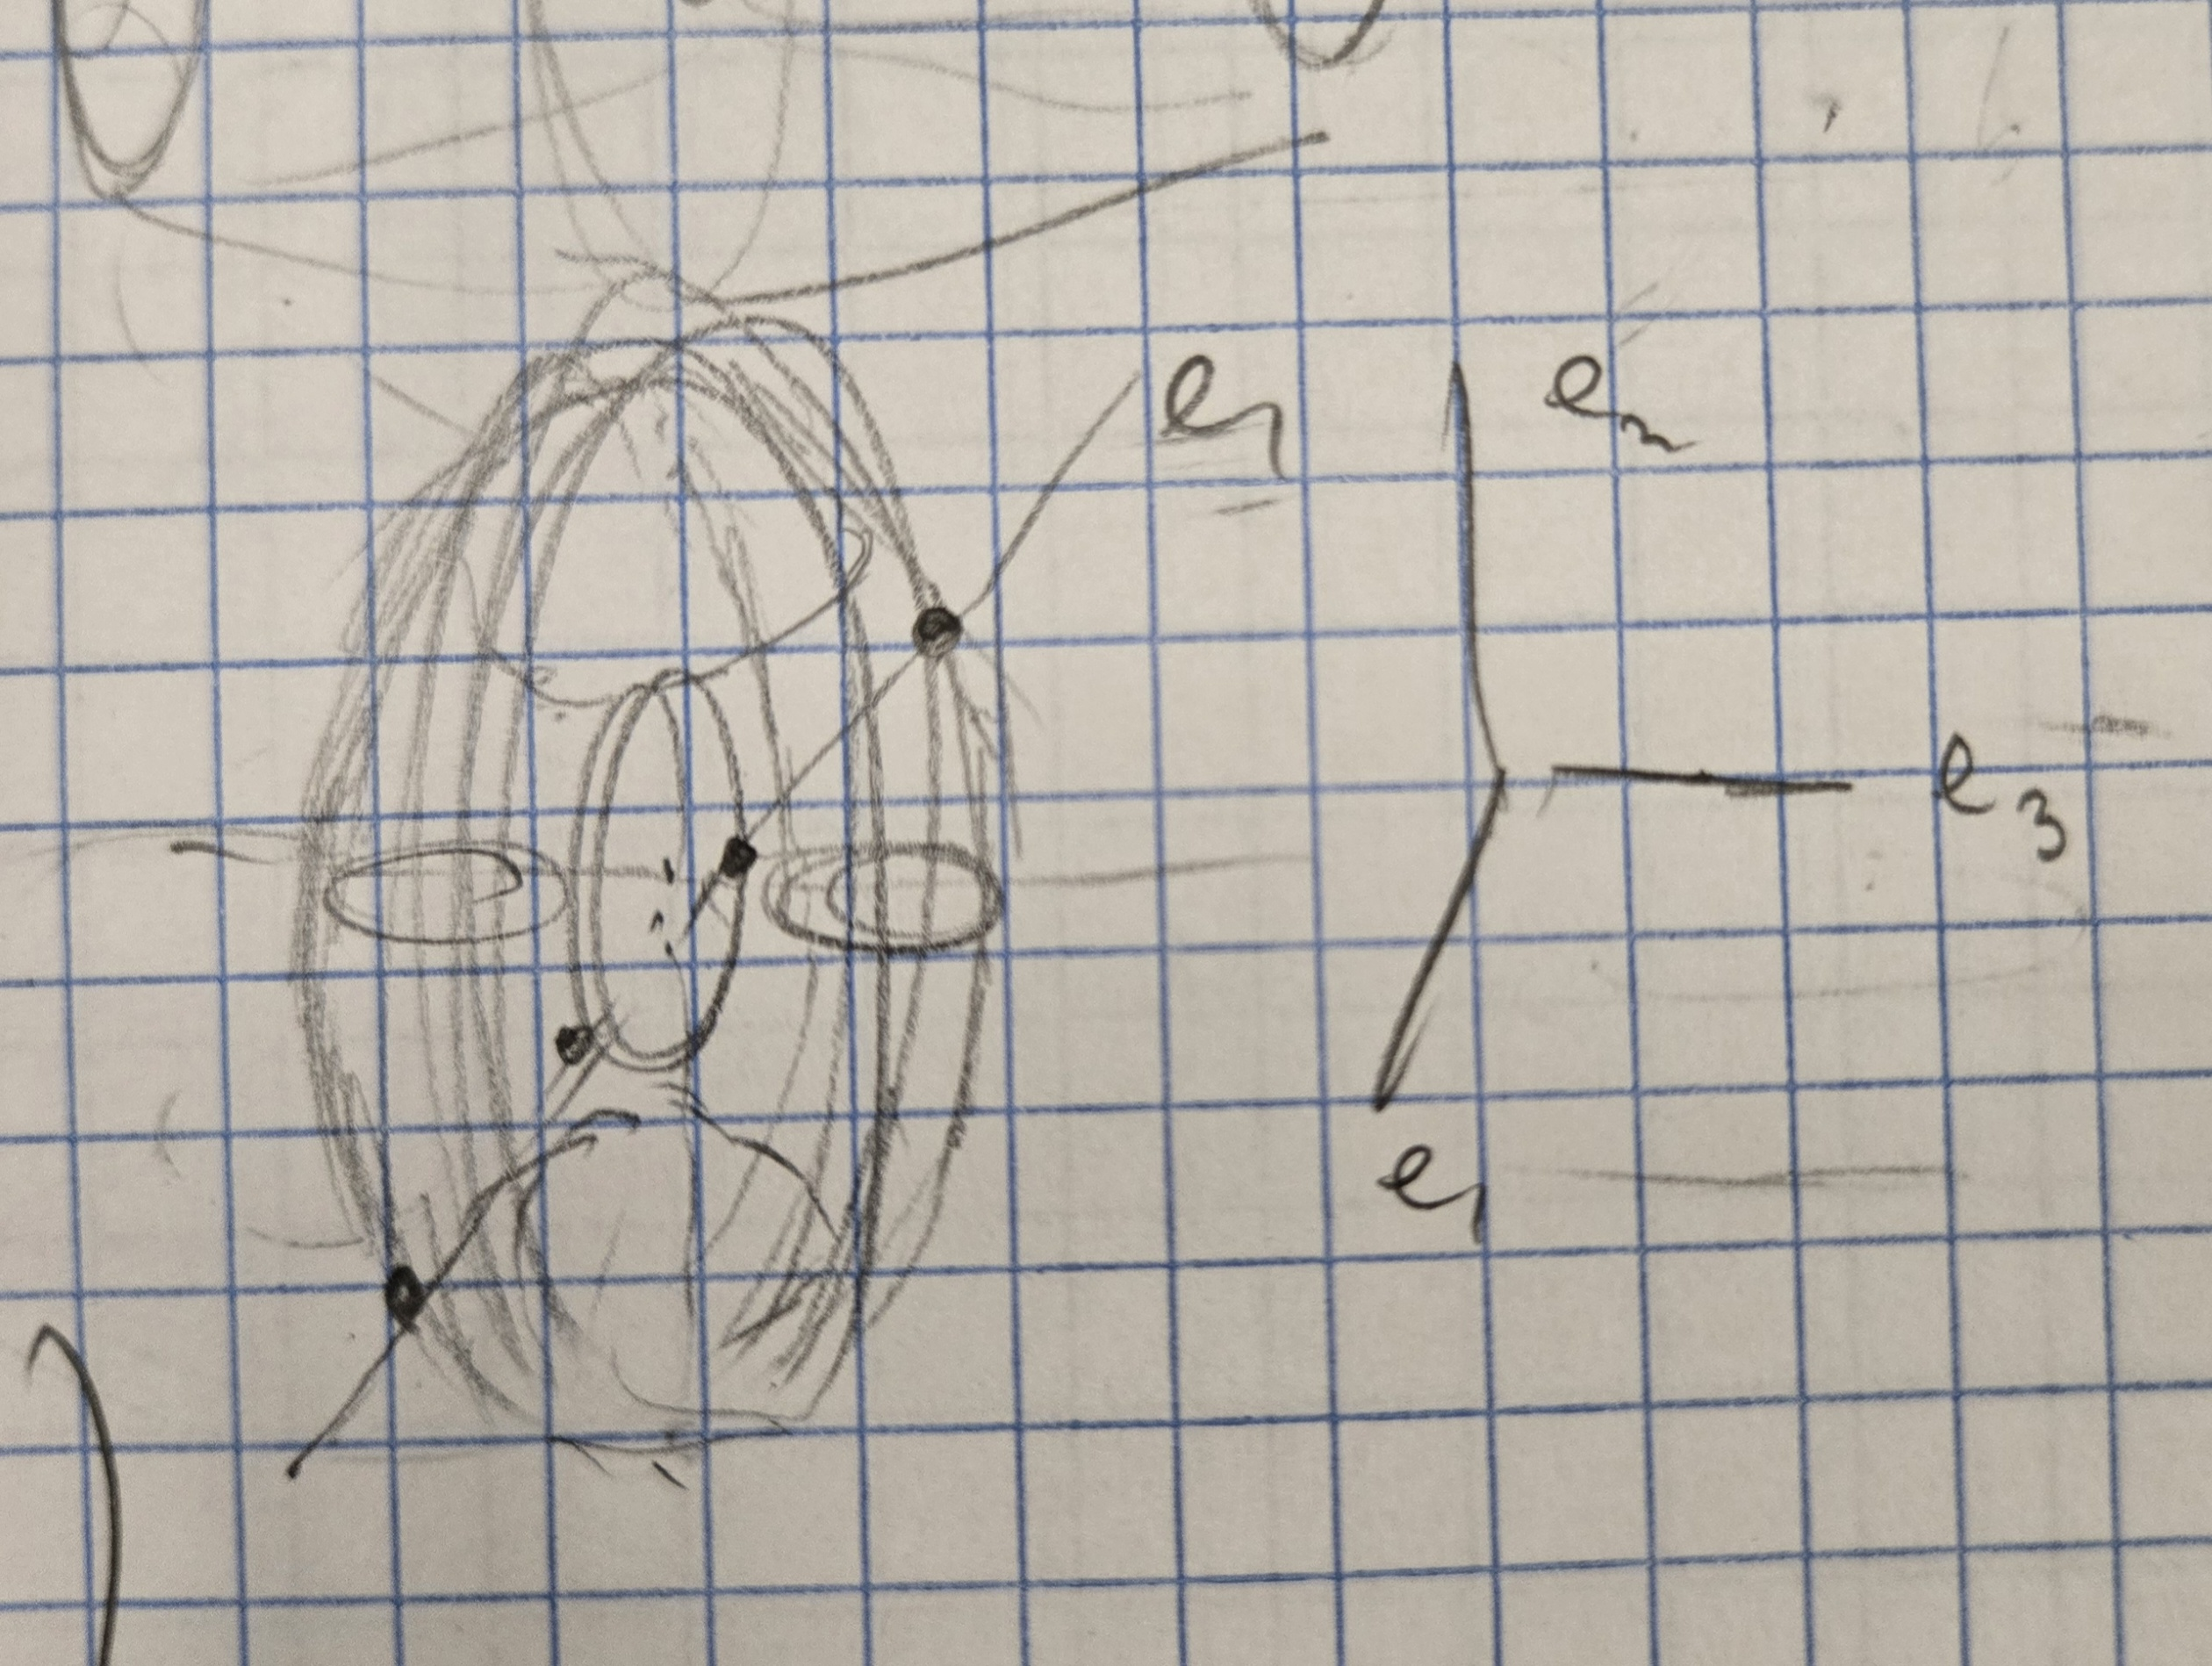
\includegraphics[width=0.5\textwidth]{torus.jpg}
  \caption{
    Torus! 
    I am visually orienting the axis in an unusual way because this is how I first conceived the geometry of this function. 
  }
  \label{fig:12_torus}
\end{figure}

\section*{Q14}
\setcounter{subsection}{0}
\subsection{}
For $(x, y) \neq (0, 0)$, 
\begin{equation} \label{eq:14_partial1}
  \Djf{1}{f}(x, y) = \frac{3x^2(x^2 + y^2) - 2x^4}{(x^2 + y^2)^2} = \frac{3x^2}{x^2 + y^2} - \frac{2x^4}{(x^2 + y^2)^2} 
\end{equation}
$\frac{3x^2}{x^2 + y^2} \leq \frac{3x^2}{x^2} = 3$ and $\frac{2x^4}{(x^2 + y^2)^2} \leq \frac{2x^4}{x^4} = 2$, so \eqref{eq:14_partial1} is bounded. 
Next, when $(x, y) \neq (0, 0)$, 
\begin{equation}  \label{eq:14_partial2}
  \Djf{2}{f}(x, y) = \frac{-2x^3 y}{(x^2 + y^2)^2}
\end{equation}
One can see \eqref{eq:14_partial2} is bounded via similar methods as above. 
Finally, one needs to check the value of the partial derivatives at $(x, y) = (0, 0)$: 
\begin{align*}
  \Djf{1}{f}(0, 0) & = \lim_{h \rightarrow 0} \frac{\frac{h^3}{h^3} - 0}{h} = 1 \\ 
  \Djf{2}{f}(0, 0) & = \lim_{h \rightarrow 0} \frac{\frac{0}{h^2} - 0}{h} = 0.
\end{align*}
So indeed, the partials are bounded everywhere. 

\subsection{}
Let $u = (u_1, u_2)$ be a unit vector, 
i.e., $u_{1}^{2} + u_{2}^{2} = 1$. 
\begin{align*}
  \Djf{u}{f}(0, 0) & = \lim_{t \rightarrow 0} \frac{\frac{t^3 u_{1}^{3}}{t^2 u_{1}^{2} + t^2 u_{2}^{2}}}{t} \\ 
                   & = \frac{u_{1}^{3}}{u_{1}^{2} + u_{2}^{2}} 
\end{align*}
and $\abs{\frac{u_{1}^{3}}{u_{1}^{2} + u_{2}^{2}}} \leq \abs{\frac{u_{1}^{3}}{u_{1}^{2}}} = \abs{u_1} \leq 1$, 
so $\Djf{u}{f}(0, 0)$ exists, and its absolute value is less or equal to 1, as was to be shown. 

\subsection{}
\textbf{(As suggested by Brandon, I will assume $\gamma(t) \neq (0, 0)$ for all $t \neq 0$).}

Away from $(0, 0)$, the partial derivatives of $f$ are continuous, so $f$ is (continuously) differentiable away from $(0, 0)$, namely with derivative 
$$f'(x, y) = \bmat{\Djf{1}{f}(x, y) & \Djf{2}{f}(x, y)} = \bmat{\frac{3x^2}{x^2 + y^2} - \frac{2x^4}{(x^2 + y^2)^2}, & \frac{-2x^3 y}{(x^2 + y^2)^2}}$$
Hence for all $t \neq 0 \in \R$, $g(t)$ is automatically differentiable by the chain rule. 
Take $t = 0$. 
Since $\gamma$ is differentiable at $0$, write $\gamma'(0) = \bmat{\alpha \\ \beta}$. 
In each coordinate, 
\begin{align*}
  \gamma_{1}(t) & = \alpha t + r_1(t) \\ 
  \gamma_2(t) & = \beta t + r_{2}(t)
\end{align*}
where $\frac{r_1(t)}{t} \rightarrow 0$ and $\frac{r_{2}(t)}{t} \rightarrow 0$ as $t \rightarrow 0$. 
Let $r_{1}(t) = t\epsilon(t)$ and $r_{2}(t) = t\eta(t)$, where $\epsilon(t), \eta(t) \rightarrow 0$ as $t \rightarrow 0$. 
Then 
\begin{align}
  \lim_{t \rightarrow 0} \frac{g(t) - g(0)}{t} 
  & = \lim_{t \rightarrow 0} \frac{1}{t} \frac{t^{3}(\alpha + \epsilon(t))^{3}}{t^2 ((\alpha + \epsilon(t))^2 + (\beta + \eta(t))^2)} \nonumber \\ 
  & = \frac{\alpha^3}{\alpha^2 + \beta^2}, \label{eq:14_atzero}
\end{align}
where $\alpha^2 + \beta^2 \neq 0$ by assumption on $\gamma'(0)$. 
This shows that $g'(0)$ exists and $g'(0) = \frac{\alpha^3}{\alpha^2 + \beta^2}$. 

Suppose $\gamma$ is $\text{C}^{1}$. 
Away from $(0, 0)$, the chain rule and the fact that both $\gamma$ and $f$ are $\text{C}^{1}$ immediately shows that $g$ is $\text{C}^{1}$. 
At $(0, 0)$, notice that in \eqref{eq:14_atzero}, $\alpha$ and $\beta$ are really functions in $t$. 
Since $\gamma$ is $\text{C}^{1}$, $\alpha$ and $\beta$ are continuous. 
The value of $g'(0)$ is just \eqref{eq:14_atzero}, so $g'(0)$ is continuous, 
which means $g$ is $\text{C}^{1}$ at $(0, 0)$ as well. 
Hence $g$ is $\text{C}^{1}$ everywhere. 

\subsection{}
If $f$ is differentiable at $(0, 0)$, then for any unit vector $u = (u_1, u_2) \in \R^2$, 
\begin{equation} \label{eq:14_dir}
 \Djf{u}{f}(0, 0) = \Djf{1}{f}(0, 0)u_1 + \Djf{2}{f}(0, 0)u_2.
\end{equation}
Take the unit vector $u = \frac{1}{\sqrt{2}}(1, 1)$. 
By prior calculations, the right hand side of \eqref{eq:14_dir} is equal to $\frac{1}{\sqrt{2}}$. 
However, the limit definition of the directional derivative gives 
$$\Djf{u}{f}(0, 0) = \lim_{t \rightarrow 0} \frac{(t 2^{-1/2})^3}{t ((t2^{-1/2})^2 + (t 2^{-1/2})^2 )} = \frac{1}{2\sqrt{2}}$$
so \eqref{eq:14_dir} doesn't hold, meaning $f$ is not differentiable at $(0, 0)$. 

\end{document}
